\documentclass{bioinfo}
\copyrightyear{2014}
\pubyear{2014}




%%% Additional Macro and command.
\usepackage{url}
\newcommand{\pkg}[1]{{\fontseries{b}\selectfont #1}}
\makeatletter
\newcommand\code{\bgroup\@makeother\_\@makeother\~\@makeother\$\@codex}
\def\@codex#1{{\normalfont\ttfamily\hyphenchar\font=-1 #1}\egroup}
\makeatother
\let\proglang=\textsf
%%% End of additional Macro and command.


\newcommand{\package}{agmus } % need that whitespace there for text flow
\usepackage{natbib}

%%% Start here.
\begin{document}


\firstpage{1}

\title[agmus]{agmus: Analyzing Genomewide Mutation and Selection pattern}
\author[
Landerer \textit{et~al}]{Cedric Landerer\,$^{1,3}$\footnote{
to whom correspondence should be addressed
},
Alex Cope\,$^{4,5}$
Russell Zaretzki\,$^{2,3}$, and
Michael Gilchrist\,$^{1,3}$
}
\address{$^{1}$
Department of Ecology and Evolutionary Biology,
$^{2}$Department of Statistics, Operations, and Management Science, and
$^{3}$National Institute for Mathematical and Biological Synthesis,
University of Tennessee, Knoxville, TN, USA,
$^{4}$Genome Science and Technology, University of Tennessee, Knoxville, TN, USA
$^{5}$Oak Ridge National Labratory, Oak Ridge, TN, USA} 
\history{Received on XXXXX; revised on XXXXX; accepted on XXXXX}

\editor{Associate Editor: XXXXXXX}

\maketitle

\begin{abstract}

\section{Summary:}
\pkg{\package} is a fast and reliable collection of codon models, estimating terms related to mutation and selection coefficients and population genetics parameters of interest from codon counts. 
The implemented models allow users to analyze sequence data and ribosome foot printing counts to estimate selection on ribosome overhead costs, nonsense error rates, and ribosome pausing times. 
In addition, \package allows for the estimation of the evolutionary average protein production rate, reflective of the environmental conditions an organism experiences. 
\package is implemented in C++ for performance increase and provides an ergonomic R interface for ease of use. 
\package also follows a generic object oriented design to allow users to extend \package and add their own models.

\section{Availability:}
\pkg{\package} and documents are freely available under the Mozilla Public License 2.0
on CRAN (\url{http://cran.r-project.org/package=cubfits}).

\section{Contact:} \href{cedric.landerer@gmail.com}{cedric.landerer@gmail.com}
\end{abstract}


\section*{Introduction}
Improvements in DNA sequencing technology and methodolgy allowed for an exponential growth in the number of publicly available genomes over the past 15 years.
This influx of data necessitates the development of computational tools which allow researchers to extract biological information.

Information regarding selection on the translation process, such as factors shaping translation efficiency and co-translational folding, can be extracted from codon usage bias (CUB) data.
CUB refers to the differential usage of synonymous codons shaped by biases in mutation and selection and can vary between organisms \citep{bulmer1991, sharp1993}.
Although CUB was first studied almost 40 years ago, many questions related to the factors shaping CUB remain open \citep{shah2011, wallace2013, gilchrist2015}.
Recent work demonstrated quantification of CUB is significantly improved in a population genetics context, which allows for both adaptive and non-adaptive evolutionary processes to be accounted for in shaping CUB.
Gilchrist et al. (2015) described a mechanistic model rooted in population genetics which accounted for selection, mutation bias, and genetic drift in quantifying CUB. 
From this model, which we call the Ribosomal Overhead Cost Stochastic Evolutionary Model of Protein Production Rates (ROC SEMPPR), relative values sof selection for translation efficiency and mutation bias within each synonymous codon family can be estimated. 
The influence of adaptive and non-adaptive processes on CUB is related to the evolutionary average protein production rate of a gene. Genes with increased protein productions rates are under higher selection for translation efficiency and are therefore composed of a higher percentage of selectively favored codons \citep{shah2011, wallace2013, gilchrist2015}. The relationship between these three biological parameters (mutation, selection, and protein production rates) allows ROC SEMPPR to order genes based on their protein production rate and therefore provide estimates of the protein production rate of each each. 

Here, we describe an open-source software that allows researchers to analyze sequence and ribosome foot-printing data. 
\package implements a Gibbs sampler within a Metropolis-Hastings Monte Carlo Markov Chain approach which allows to incorporate prior knowledge and easy sampling from the posterior distribution to estimate parameter uncertainty. 
Currently, \package provides three models to analyze codon counts obtained from coding sequences or ribosome foot-printing experiments. 
The ROC model implements the work presented by Gilchrist et al. (2015), selection on \underline{r}ibosome \underline{o}verhead \underline{c}ost and inferring protein synthesis rates.
The NSE model is focused on the estimation of \underline{n}on-\underline{s}ense \underline{e}rror rates and accounts for the position of a codon in the sequence, where codons found later in the sequence are assumed to be under stronger selection against non-sense errors.
Both model allow for the separation of effects of mutation and selection based on gene ordering by protein synthesis rate.
Furthermore, \package implements a RFP model to extract information on ribosome pausing times from \underline{r}ibosome \underline{f}oot-\underline{p}rinting data. 
All models share the insight that selection for translation efficiency scales with protein production rate and therefore share the ability to order genes based on protein production rate. 
\package also extends all provided models with a mixture component, allowing for intra-genomic variation in mutation and selection as it can be caused by hybridization or introgression events.

\begin{figure*}[!tpb]
\centering
 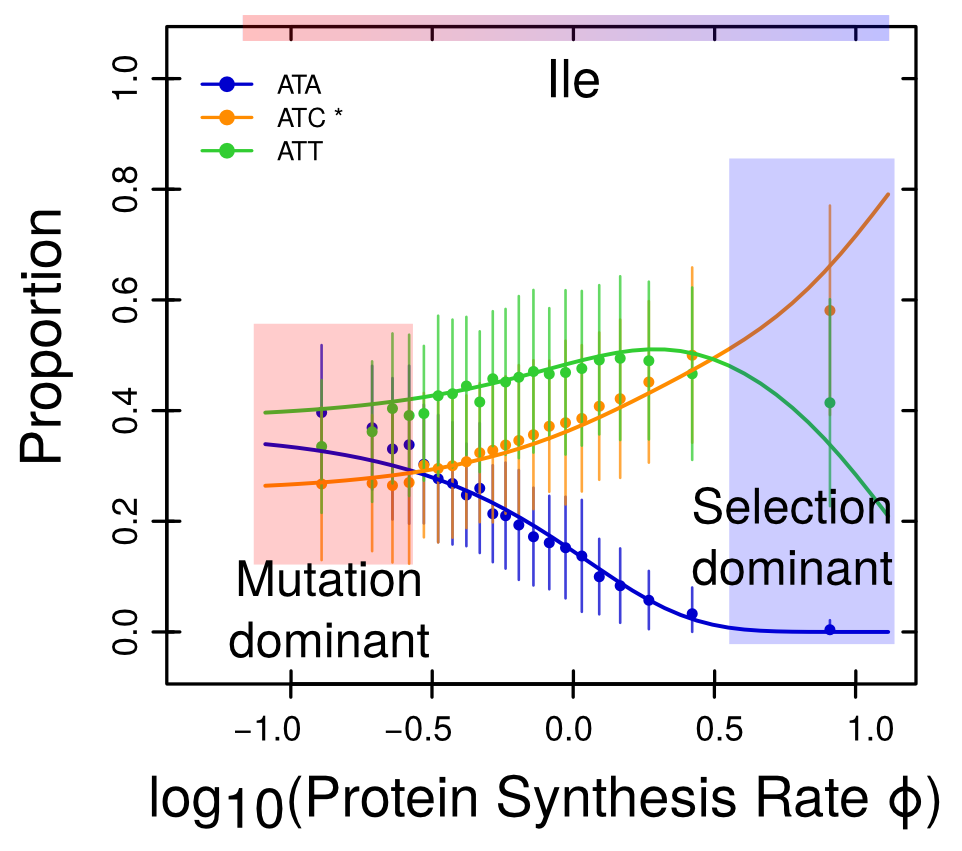
\includegraphics[width=3in]{expl_model.png}
\vspace{-0.2cm}
\caption{\textbf{Package overview and plotting functionality.} A) \package workflow and class dependencies. B) Comparison of mutation bias estimated for the different mixture distributions within a data-set. C) CUB varies with gene expression. Indicated in red and blue, regions with mutation and selection dominant, receptively (not part of the plotting). 
}
\label{fig:plotbin}
\end{figure*}

\section*{Features}
\package provides an interface written in R \citep{rcore}, a freely available programming language noted for its ease of use for even inexperienced programmers. As a result, \package is accessible to researchers with minimal computational experience. The framework provides an convenient interface designed to allow researchers to analyze their data swiftly without the need for long preprocessing of data sets. Generally, the only input needed for fitting a model to the data are protein-coding nucleotide sequences in the form of a FASTA file or a flat-file containing codon counts obtained from ribosome foot-printing experiments. If available, users may also provide empirically estimated values of gene expression as additional guide for the model. However, this is not required.
\package also provides visualization functionality, including plot functions to compare parameter estimates for different mixture distributions, functions to display codon usage patterns and diagnostic functions to assess the goodness of fit (Figure 1).

\subsubsection*{Mixture distributions}
Mixture distributions are commonly used when a data set is comprised of sub-populations, which can be described by distinguishable distributions of parameters \citep{gelman2013}. \package extends all implemented models with the ability to utilize mixture distributions for all population parameters like mutation and selection. As all implemented model contain gene specific parameters (e.g. protein production rate) in addition to population specific parameters (e.g. mutation) we extended the mixture approach implemented in \package to incorporate the need for a gene specific parameter. Therefore, the protein production rate of each gene is estimated assuming it in each possible mixture distribution. This approach allows genes to be categorized based on differences in codon usage patterns, making \package ideal to ask questions about intra-genomic or even within-gene heterogeneity in mutation and selection patterns. 

\subsubsection*{C++ to improve computational efficiency}
Although \package is provided as an R package, the software is completely implemented in C++ and can be, if desired, compiled as a standalone software.
Since R does not provide a native C++ support; we utilized the R package Rcpp \citep{rcpp_package}. 
Rcpp provides a module structure allowing the exposure of whole C++ classes to R. 
This minimizes data transfer between the R environment and the C++ core, resulting in improved computational performance and allowed for a fully object oriented code design. 
The runtime of \package scales as expected linear with genome size and number of iterations, and quadratic with the number of mixture distributions in the data set. The quadratic increase in the number of mixture distributions is explained by the necessity to estimate the protein production rate for each gene in each mixture distribution, as it is a gene specific parameter.  

\subsubsection*{Available models}
\package currently contains three codon models analyzing codon usage patterns to estimate biologically relevant parameters such as strength and direction of mutation bias and protein production rate. 
ROC SEMPPER \cite{gilchrist2015} and NSE SEMPER (unpublished) analyze sequence data and extract information about ribosome overhead cost and nonsense error rate of synonymous codons, respectively. 
RFP SEMPPER estimates ribosome pausing time from ribosome foot-printing counts.

%\subsubsection*{Writing extensions}
Users are welcome and encouraged to incorporate their own codon models into \package. The object-oriented paradigm of C++ allowed for the implementation of a general framework for creating new models to analyze genomic data. All implemented models in \package are encapsulated such that they share certain commonalities. This allows for the creation of new models within the same framework. Generally, these models can be added by creating appropriate subclasses of the Parameter and Model classes provided by the current framework. These subclasses should include the additional functionality required for these models. 

\bibliographystyle{natbib}
\bibliography{bioinfo}
\end{document}
